\ifx\wholebook\relax \else
% ------------------------ 

\documentclass{article}
%------------------- Other types of document example ------------------------
%
%\documentclass[twocolumn]{IEEEtran-new}
%\documentclass[12pt,twoside,draft]{IEEEtran}
%\documentstyle[9pt,twocolumn,technote,twoside]{IEEEtran}
%
%-----------------------------------------------------------------------------
%%
% loading packages
%
\newif\ifpdf
\ifx\pdfoutput\undefined % We're not running pdftex
  \pdffalse
\else
  \pdftrue
\fi
%
%
\ifpdf
  \RequirePackage[pdftex,%
            CJKbookmarks,%
       bookmarksnumbered,%
              colorlinks,%
          linkcolor=blue,%
              hyperindex,%
        plainpages=false,%
       pdfstartview=FitH]{hyperref}
\else
  \RequirePackage[dvipdfm,%
             CJKbookmarks,%
        bookmarksnumbered,%
               colorlinks,%
           linkcolor=blue,%
               hyperindex,%
         plainpages=false,%
        pdfstartview=FitH]{hyperref}
  \AtBeginDvi{\special{pdf:tounicode GBK-EUC-UCS2}} % GBK -> Unicode
\fi
\usepackage{hyperref}

% other packages
%-----------------------------------------------------------------------------
\usepackage{graphicx, color}
\usepackage{CJK}
%
% for programming 
%
\usepackage{verbatim}
\usepackage{listings}


\lstdefinelanguage{Smalltalk}{
  morekeywords={self,super,true,false,nil,thisContext}, % This is overkill
  morestring=[d]',
  morecomment=[s]{"}{"},
  alsoletter={\#:},
  escapechar={!},
  literate=
    {BANG}{!}1
    {UNDERSCORE}{\_}1
    {\\st}{Smalltalk}9 % convenience -- in case \st occurs in code
    % {'}{{\textquotesingle}}1 % replaced by upquote=true in \lstset
    {_}{{$\leftarrow$}}1
    {>>>}{{\sep}}1
    {^}{{$\uparrow$}}1
    {~}{{$\sim$}}1
    {-}{{\sf -\hspace{-0.13em}-}}1  % the goal is to make - the same width as +
    %{+}{\raisebox{0.08ex}{+}}1		% and to raise + off the baseline to match -
    {-->}{{\quad$\longrightarrow$\quad}}3
	, % Don't forget the comma at the end!
  tabsize=2
}[keywords,comments,strings]

\lstloadlanguages{C++, Lisp, Haskell, Python, Smalltalk}

% ======================================================================

\def\BibTeX{{\rm B\kern-.05em{\sc i\kern-.025em b}\kern-.08em
    T\kern-.1667em\lower.7ex\hbox{E}\kern-.125emX}}

\newtheorem{theorem}{Theorem}

%
% mathematics
%
\newcommand{\be}{\begin{equation}}
\newcommand{\ee}{\end{equation}}
\newcommand{\bmat}[1]{\left( \begin{array}{#1} }
\newcommand{\emat}{\end{array} \right) }
\newcommand{\VEC}[1]{\mbox{\boldmath $#1$}}

% numbered equation array
\newcommand{\bea}{\begin{eqnarray}}
\newcommand{\eea}{\end{eqnarray}}

% equation array not numbered
\newcommand{\bean}{\begin{eqnarray*}}
\newcommand{\eean}{\end{eqnarray*}}

\RequirePackage{CJK,CJKnumb,CJKulem,CJKpunct}
% we use CJK as default environment
\AtBeginDocument{\begin{CJK*}{GBK}{song}\CJKtilde\CJKindent\CJKcaption{GB}}
\AtEndDocument{\clearpage\end{CJK*}}

%
% loading packages
%

\RequirePackage{ifpdf}

%
%
\ifpdf
  \RequirePackage[pdftex,%
       bookmarksnumbered,%
              colorlinks,%
          linkcolor=blue,%
              hyperindex,%
        plainpages=false,%
       pdfstartview=FitH]{hyperref}
\else
  \RequirePackage[dvipdfm,%
        bookmarksnumbered,%
               colorlinks,%
           linkcolor=blue,%
               hyperindex,%
         plainpages=false,%
        pdfstartview=FitH]{hyperref}
\fi
\usepackage{hyperref}

% other packages
%--------------------------------------------------------------------------
\usepackage{graphicx, color}
\usepackage{subfig}

\usepackage{amsmath, amsthm, amssymb} % for math
\usepackage{exercise} % for exercise

%
% for programming 
%
\usepackage{verbatim}
\usepackage{listings}
%\usepackage{algorithmic} %old version; we can use algorithmicx instead
\usepackage{algorithm} 
\usepackage[noend]{algpseudocode} %for pseudo code, include algorithmicsx automatically
\usepackage{makeidx} % for index support


\lstdefinelanguage{Smalltalk}{
  morekeywords={self,super,true,false,nil,thisContext}, % This is overkill
  morestring=[d]',
  morecomment=[s]{"}{"},
  alsoletter={\#:},
  escapechar={!},
  literate=
    {BANG}{!}1
    {UNDERSCORE}{\_}1
    {\\st}{Smalltalk}9 % convenience -- in case \st occurs in code
    % {'}{{\textquotesingle}}1 % replaced by upquote=true in \lstset
    {_}{{$\leftarrow$}}1
    {>>>}{{\sep}}1
    {^}{{$\uparrow$}}1
    {~}{{$\sim$}}1
    {-}{{\sf -\hspace{-0.13em}-}}1  % the goal is to make - the same width as +
    %{+}{\raisebox{0.08ex}{+}}1		% and to raise + off the baseline to match -
    {-->}{{\quad$\longrightarrow$\quad}}3
	, % Don't forget the comma at the end!
  tabsize=2
}[keywords,comments,strings]

\lstloadlanguages{C++, Lisp, Haskell, Python, Smalltalk}

% ======================================================================

\def\BibTeX{{\rm B\kern-.05em{\sc i\kern-.025em b}\kern-.08em
    T\kern-.1667em\lower.7ex\hbox{E}\kern-.125emX}}

%
% mathematics
%
\newcommand{\be}{\begin{equation}}
\newcommand{\ee}{\end{equation}}
\newcommand{\bmat}[1]{\left( \begin{array}{#1} }
\newcommand{\emat}{\end{array} \right) }
\newcommand{\VEC}[1]{\mbox{\boldmath $#1$}}

% numbered equation array
\newcommand{\bea}{\begin{eqnarray}}
\newcommand{\eea}{\end{eqnarray}}

% equation array not numbered
\newcommand{\bean}{\begin{eqnarray*}}
\newcommand{\eean}{\end{eqnarray*}}

\newtheorem{theorem}{Theorem}[section]
\newtheorem{lemma}[theorem]{Lemma}
\newtheorem{proposition}[theorem]{Proposition}
\newtheorem{corollary}[theorem]{Corollary}


\setcounter{page}{1}

\begin{document}

\fi
%--------------------------

% ================================================================
%                 COVER PAGE
% ================================================================

\title{B-Trees with Functional and imperative implementation}

\author{Liu~Xinyu
\thanks{{\bfseries Liu Xinyu } \newline
  Email: liuxinyu95@gmail.com \newline}
%  Tel:   +86-1305-196-8666 \newline}
  }

\markboth{B-Trees}{Imperative and Functional}

\maketitle

\ifx\wholebook\relax
\chapter{B-Trees with Functional and imperative implementation}

\section{abstract}
\else
\begin{abstract}
\fi
B-Tree is introduced by CLRS book as one of the advanced data
structures. It is important to the modern file systems, some of them
are implemented based on B+ tree, which is extended from B-tree.
It is also widely used in many database systems. This post provides
some implementation of B-trees both in imperative way as described in
CLRS books and in functional way with a kind of modify-and-fix
approach. There are multiple programming languages used, including
C++, Haskell, Python and Scheme/Lisp.

There may be mistakes in the post, please feel free to point out.

This post is generated by \LaTeXe, and provided with GNU FDL(GNU Free Documentation License).
Please refer to http://www.gnu.org/copyleft/fdl.html for detail.

\ifx\wholebook\relax \else
\end{abstract}
\fi

\vspace{3cm}
{\bfseries Keywords:} B-Trees

%{\bfseries Corresponding Author:} Liu Xinyu

\maketitle

% ================================================================
%                 Introduction
% ================================================================
\section{Introduction}
\label{introduction}

In CLRS book, B-tree is introduced with the the problem of how to access a
large block of data on magnetic disks or secondary storage devices\cite{CLRS}.
B-tree is commonly used in databases and filesystems.

It is also helpful to understand B-tree as a generalization of balanced binary
search tree\cite{wiki-b-tree}.

Refer to the Figure \ref{fig:btree-example}, It is easy to found the difference
and similarity of B-tree regarding to binary search tree.

\begin{figure}[htbp]
       \begin{center}
	\includegraphics[scale=0.5]{img/btree-example.ps}
        \caption{An example of B-Tree} \label{fig:btree-example}
       \end{center}
\end{figure}

Let's review the definition of binary search tree \cite{lxy-bst}.

A binary search tree is 
\begin{itemize}
\item either an empty node;
\item or a node contains 3 parts, a value, a left child which is a
binary search tree and a right child which is also a binary search tree.
\end{itemize}

An it satisfies the constraint that.
\begin{itemize}
\item all the values in left child tree is less than the value of of this node;
\item the value of this node is less than any values in its right child tree.
\end{itemize}

The constraint can be represented as the following. for any node $n$,
it satisfies the below equation.

\begin{equation}
\forall x \in LEFT(n), \forall y \in RIGHT(n) \\
\Rightarrow VALUE(x)<VALUE(n)<VALUE(y)
\end{equation}

If we extend this definition to allow multiple keys and children, we get the 
below definition.

A B-tree is 
\begin{itemize}
\item either an empty node;
\item or a node contains $n$ keys, and $n+1$ children, each child is
also a B-Tree, we denote these keys and childrens as $key_1, key_2,
..., key_n$ and $c_1, c_2, ..., c_n, c_{n+1}$.
\end{itemize}

Figure \ref{fig:btree-node} illustrates a B-Tree node.

\begin{figure}[htbp]
       \begin{center}
	\includegraphics[scale=0.5]{img/btree-node.ps}
        \caption{A B-Tree node} \label{fig:btree-node}
       \end{center}
\end{figure}

The keys and children in a node satisfy the following order constraints.

\begin{itemize}
\item Keys are stored in nondecreasing order. that is $key_1 \leq
key_2 \leq ... \leq key_n$;
\item for each $key_i$, all values stored in child $c_i$ are no bigger 
than $key_i$, while all values stored in child $c_{i+1}$ are no less
than $key_i$.
\end{itemize}

The constraints can be representd as in equation ref{eq:btree-order}
as well.

\begin{equation}
\forall x_i \in c_i, i=0, ..., n, \Rightarrow x_1 \leq key_1 \leq
x_2 \leq key_2 \leq ... \leq x_n \leq key_n \leq x_{n+1}
\end{equation}

Finally, if we added some constraints to make the tree balanced, we get the
complete definition of B-tree.

\begin{itemize}
\item All leaves have the same depth;
\item We define an integral number, $t$, as the {\em minumum degree} of a 
B-tree;
    \begin{itemize}
        \item each node can have at most $2t-1$ keys;
        \item each node can have at least $t-1$ keys, except the root;
    \end{itemize}
\end{itemize}

In this post, I'll first introduce How to generate B-trees by insertion
algorithm. Two different methods will be explained. One method is discussed in CLRS
book, the other is a kind of modify-fix approach which quite similar to the
algorithm Okasaki used in red-black tree\cite{okasaki-rbtree}. This method
is also discussed in wikipedia\cite{wiki-b-tree}. After that, how to delete
element from B-tree is explained. As the last part, algorithm for searching 
in B-tree is also provided.

This article provides example implementation in C, C++, Haskell, Python, and 
Scheme/Lisp languages. 

All source code can be downloaded in appendix \ref{appendix}, please 
refer to appendix for detailed information about build and run.

% ================================================================
%                 Definition
% ================================================================
\section{Definition}
\label{btree-definition}

Similar as Binary search tree, B-tree can be defined recursively.
Because there are multiple of keys and children, a collection container
can be used to store them.

\subsection*{Definition of B-tree in C++}
ISO C++ support using const integral number as template parameter.
This feature can used to define B-tree with different minimum degree
as different type.

\lstset{language=C++}
\begin{lstlisting}
// t: minimum degree of B-tree
template<class K, int t>
struct BTree{
  typedef K key_type;
  typedef std::vector<K> Keys;
  typedef std::vector<BTree*> Children;

  BTree(){}

  ~BTree(){
    for(typename Children::iterator it=children.begin();
        it!=children.end(); ++it)
      delete (*it);
  }

  bool full(){ return keys.size() == 2*t-1; }

  bool leaf(){
    return children.empty();
  }

  Keys keys;
  Children children; 
};
\end{lstlisting}

In order to support ramdom access to keys and children, the
inner data structure uses STL vector. The node will recursively
release all its children. and a two simple auxiliary member
functions ``full'' and ``leaf'' are provided to test if a node
is full or is a leaf node.

\subsection*{Definition of B-tree in Python}

If the minimum degree is 2, the B-tree is commonly called as 2-3-4 tree.
For illustration purpose, I set 2-3-4 tree as default.

\lstset{language=Python}
\begin{lstlisting}
TREE_2_3_4 = 2 #by default, create 2-3-4 tree

class BTreeNode:
    def __init__(self, t=TREE_2_3_4, leaf=True):
        self.leaf = leaf
        self.t = t
        self.keys = [] #self.data = ...
        self.children = []
\end{lstlisting}

It's quite OK for B-tree not only store keys, but also store satelite data.
However, satelite data is omitted in this post.

Also there are some auxiliary member functions defined

\begin{lstlisting}
class BTreeNode:
    #...
    def is_full(self):
        return len(self.keys) == 2*self.t-1
\end{lstlisting}

This member function is used to test if a node is full.

\subsection*{Definition of B-tree in Haskell}
In Haskell, record syntax is used to define BTree, so that keys and children 
can be access easily later on. Some auxiliary functions are also provided.

\lstset{language=Haskell}
\begin{lstlisting}
data BTree a = Node{ keys :: [a]
                   , children :: [BTree a]
                   , degree :: Int} deriving (Eq, Show)

-- Auxiliary functions
empty deg = Node [] [] deg

full::BTree a -> Bool
full tr = (length $ keys tr) > 2*(degree tr)-1
\end{lstlisting} %$

\subsection*{Definition of B-tree in Scheme/Lisp}
TODO: ...

% ================================================================
%                 Insertion
% ================================================================
\section{Insertion}
\label{btree-insertion}
Insertion is the basic operation to B-tree, a B-tree can be created by inserting
keys repeatly. The essential idea of insertion is similar to the binary
search tree. If the keys to be inserted is x, we examine the keys in a 
node to find a position where all the keys on the left are less than x,
while all the keys on the right hand are greater than x. after that
we can recursively insert x to the child node at this position.

However, this basic idea need to be fine tuned. The first thing is what
the recursion termination criteria is. This problem can be easily solved
by define the rule that, in case the node to be inserted is a leaf node.
We needn't do inserting recursively. This is because leaf node don't have
children at all. We can just put the x between all left hand keys and 
right hand keys, which cause the keys number of a leaf node increased by one.

The second thing is how to keep the balance properties of a B-tree when
inserting. if a leaf has already $2t-1$ keys, it will break the rule of '
each node can has at most $2t-1$ keys' after we insert x to it. Below
sections will show 2 major methods to solve this problem. 

%=========================================================================
%       Splitting
%=========================================================================
\subsection{Splitting}
\label{split}
Regarding to the problem of insert a key to a node, which has already
$2t-1$ keys, one solution is to split the node before insertion.

In this case, we can devide the node into 3 parts as shown in 
Figure \ref{fig:node-split}. the left part contains first $t-1$ keys
and $t$ children, while the right part contains the last $t-1$ keys
and $t$ children. Both left part and right part are valid B-tree
nodes. the middle part is just the $t$-th key. It is pushed up
to its parent node (if it already root node, then the $t$-th key,
with 2 children turn be the new root).

\begin{figure}[htbp]
       \begin{center}
       	  \includegraphics[scale=0.5]{img/split-node-before.ps}

          a. Before split,

          \includegraphics[scale=0.5]{img/split-node-after.ps}

          b. After split, 
        \caption{Split node} \label{fig:node-split}
       \end{center}
\end{figure}

\subsubsection{Imperative splitting}
If we skip the disk accessing part as explained in \cite{CLRS}. The 
imperative splitting algorithms can be shown as below.

\begin{algorithmic}[1]
\Procedure{B-TREE-SPLIT-CHILD}{$node, i$}
  \State $x \leftarrow CHILDREN(node)[i]$
  \State $y \leftarrow CREATE-NODE()$
  \State $INSERT(KEYS(node), i, KEYS(x)[t])$
  \State $INSERT(CHILDREN(node), i+1, y)$
  \State $KEYS(y) \leftarrow KEYS(x)[t+1 ... 2t-1]$
  \State $KEYS(x) \leftarrow KEYS(x)[1 ... t-1]$
  \If{$y$ is not leaf}
    \State $CHILDREN(y) \leftarrow CHILDREN(x)[t+1 ... 2t]$
    \State $CHILDREN(x) \leftarrow CHILDREN(x)[1 ... t]$
  \EndIf
\EndProcedure
\end{algorithmic}

This algorithm take 2 parameters, one is a B-tree node, the other
is the index to indicate which child of this node will be split.

\subsubsection*{Split implemented in C++}
The algorithm can be implemented in C++ as a member function of
B-tree node.

\lstset{language=C++}
\begin{lstlisting}
template<class K, int t>
struct BTree{

  //...

  void split_child(int i){
    BTree<K, t>* x = children[i];
    BTree<K, t>* y = new BTree<K, t>();
    keys.insert(keys.begin()+i, x->keys[t-1]);
    children.insert(children.begin()+i+1, y);
    y->keys = Keys(x->keys.begin()+t, x->keys.end());
    x->keys = Keys(x->keys.begin(), x->keys.begin()+t-1);
    if(!x->leaf()){
      y->children = Children(x->children.begin()+t, x->children.end());
      x->children = Children(x->children.begin(), x->children.begin()+t);
    }
  }
\end{lstlisting}

\subsubsection*{Split implemented in Python}
We can define splitting operation as a member method of B-tree
as the following.

\lstset{language=Python}
\begin{lstlisting}
class BTreeNode:
    #...
    def split_child(self, i):
        t = self.t
        x = self.children[i]
        y = BTreeNode(t, x.leaf)
        self.keys.insert(i, x.keys[t-1])
        self.children.insert(i+1, y)
        y.keys = x.keys[t:]
        x.keys = x.keys[:t-1]
        if not y.leaf:
            y.children = x.children[t:]
            x.children = x.children[:t]
\end{lstlisting}

\subsubsection{Functional splitting}

For functional algorithm, splitting will return a tuple, which contains the
left part and right as B-Trees, along with a key.

\begin{algorithmic}[1]
\Function{B-TREE-SPLIT}{$node$}
  \State $ks \leftarrow KEYS(node)[1 ... t-1]$
  \State $ks' \leftarrow KEYS(node)[t+1 ... 2t-1]$
  \If{$node$ is not leaf}
    \State $cs \leftarrow CHILDREN(node)[1 ... t]$
    \State $cs' \leftarrow CHILDREN(node)[t ... 2t]$
  \EndIf
  \State \Return $(CREATE-B-TREE(ks, cs), KEYS(node)[t], CREATE-B-TREE(ks', cs'))$
\EndFunction
\end{algorithmic}

\subsubsection*{Split implemented in Haskell}
Haskell prelude provide take/drop functions to get the part
of the list. These functions just returns empty list if the 
list passed in is empty. So there is no need to test if
the node is leaf.

\lstset{language=Haskell}
\begin{lstlisting}
split :: BTree a -> (BTree a, a, BTree a)
split (Node ks cs t) = (c1, k, c2) where
    c1 = Node (take (t-1) ks) (take t cs) t
    c2 = Node (drop t ks) (drop t cs) t
    k  = head (drop (t-1) ks)
\end{lstlisting}

\subsubsection*{Split implemented in Scheme/Lisp}
TODO: ...

%=========================================================================
%       Split before insertion
%=========================================================================
\subsection{Split before insert method}
\label{split before insertion}

Note that the split solution will push a key up to its parent node,
It is possible that the parent node be full if it has already 
$2t-1$ keys.

Regarding to this issue, the CLRS book provides a solution to check 
every node from root along the path until leaf, in case there is a 
node in this path is full. the split is applied. Since the parent
of this node has been examined except the root node, which ensure
the parent node has less than $2t-1$ keys, the pushing up of one
key won't make the parent full. This approach need only a single
pass down the tree without need of any back-tracking.

The main insert algorithm will first check if the root node need
split. If yes, it will create a new node, and set the root as the 
only child, then performs splitting. and set the new node as the
root. After that, the algorithm will try to insert the key to the
non-full node.

\begin{algorithmic}[1]
\Function{B-TREE-INSERT}{$T, k$}
  \State $r \leftarrow T$
  \If{$r$ is full}
    \State $s \leftarrow CREATE-NODE()$
    \State $APPEND(CHILDREN(s), r)$
    \State $B-TREE-SPLIT-CHILD(s, 1)$
    \State $r \leftarrow s$
  \EndIf
  \State $B-TREE-INSERT-NONFULL(r, k)$
  \State \Return $r$
\EndFunction
\end{algorithmic}

The algorithm $B-TREE-INSERT-NONFUL$ assert that the node passed in
is not full. If it is a leaf node, the new key is just inserted to 
the proper postion based on its order. If it is a branch node. The algorithm
finds a proper child node to which the new key will be inserted.
If this child node is full, the splitting will be performed firstly.

\begin{algorithmic}[1]
\Procedure{B-TREE-INSERT-NONFUL}{$T, k$}
  \If{$T$ is leaf}
    \State $i \leftarrow 1$
    \While{$i \leq LENGTH(KEYS(T))$ and $k>KEYS(T)[i]$}
      \State $i \leftarrow i+1$
    \EndWhile
    \State $INSERT(KEYS(T), i, k)$
  \Else
    \State $i \leftarrow LENGTH(KEYS(T))$
    \While{$i>1 and k < KEYS(T)[i]$}
      \State $i \leftarrow i-1$
    \EndWhile
    \If{$CHILDREN(T)[i]$ is full}
      \State $B-TREE-SPLIT-CHILD(T, i)$
      \If{$k > KEYS(T)[i]$}
        \State $i \leftarrow i+1$
      \EndIf
    \EndIf
    \State $B-TREE-INSERT-NONFULL(CHILDREN(T)[i], k)$
  \EndIf
\EndProcedure
\end{algorithmic}

Note that this algorithm is actually recursive. Consider B-tree typically
has minimum degree t relative to magnetic disk structure, and it is balanced 
tree, Even small depth can support huge amount of data 
(with $t=10$, maximum to 10 billion data can be stored in a B-tree with height of 10).
Of course it is easy to eliminate the recursive call to improve the algorithm.

In the below language specific implementations, I'll eliminate recursion in 
C++ program, and show the recurisve version in Pythono program.

\subsubsection*{Insert implemented in C++}
The main insert program in C++ examine if the root is full and performs splitting
accordingly. Then it will call insert\_nonfull to do the further process.

\lstset{language=C++}
\begin{lstlisting}
template<class K, int t>
BTree<K, t>* insert(BTree<K, t>* tr, K key){
  BTree<K, t>* root(tr);
  if(root->full()){
    BTree<K, t>* s = new BTree<K, t>();
    s->children.push_back(root);
    s->split_child(0);
    root = s;
  }
  return insert_nonfull(root, key);
}
\end{lstlisting}

The resursion is eliminated in insert\_nonfull function. If the current
node is leaf, it will call orderred\_insert to insert the key to the correct
position. If it is branch node, the program will find the proper child
tree and set it as the current node in next loop. Splitting is performed
if the child tree is full.

\begin{lstlisting}
template<class K, int t>
BTree<K, t>* insert_nonfull(BTree<K, t>* tr, K key){
  typedef typename BTree<K, t>::Keys Keys;
  typedef typename BTree<K, t>::Children Children;

  BTree<K, t>* root(tr);
  while(!tr->leaf()){
    unsigned int i=0;
    while(i < tr->keys.size() && tr->keys[i] < key)
      ++i;
    if(tr->children[i]->full()){
      tr->split_child(i);
      if(key > tr->keys[i])
        ++i;
    }
    tr = tr->children[i];
  }
  orderred_insert(tr->keys, key);
  return root;
}
\end{lstlisting}

Where the orderred\_insert is defined as the following.

\begin{lstlisting}
template<class Coll>
void orderred_insert(Coll& coll, typename Coll::value_type x){
  typename Coll::iterator it = coll.begin();
  while(it != coll.end() && *it < x)
    ++it;
  coll.insert(it, x);
}
\end{lstlisting}

For convenience, I defined auxiliar functions to convert a
list of keys into the B-tree.

\begin{lstlisting}
template<class T>
T* insert_key(T* t, typename T::key_type x){
  return insert(t, x);
}

template<class Iterator, class T>
T* list_to_btree(Iterator first, Iterator last, T* t){
  return std::accumulate(first, last, t,
                         std::ptr_fun(insert_key<T>));
}
\end{lstlisting}

In order to print the result as human readable string, a recursive
convert function is provided.

\begin{lstlisting}
template<class T>
std::string btree_to_str(T* tr){
  typename T::Keys::iterator k;
  typename T::Children::iterator c;

  std::ostringstream s;
  s<<"(";
  if(tr->leaf()){
    k=tr->keys.begin();
    s<<*k++;
    for(; k!=tr->keys.end(); ++k)
      s<<", "<<*k;
  }
  else{
    for(k=tr->keys.begin(), c=tr->children.begin();
        k!=tr->keys.end(); ++k, ++c)
      s<<btree_to_str(*c)<<", "<<*k<<", ";
    s<<btree_to_str(*c);
  }
  s<<")";
  return s.str();
}
\end{lstlisting}

With all the above defined program, some simple test cases can be
fed to verfiy the program.

\begin{lstlisting}
const char* ss[] = {"G", "M", "P", "X", "A", "C", "D", "E", "J", "K", \
                    "N", "O", "R", "S", "T", "U", "V", "Y", "Z"};
BTree<std::string, 2>* tr234=list_to_btree(ss, ss+sizeof(ss)/sizeof(char*),
                                           new BTree<std::string, 2>);
std::cout<<"2-3-4 tree of ";
std::copy(ss, ss+sizeof(ss)/sizeof(char*), 
          std::ostream_iterator<std::string>(std::cout, ", "));
std::cout<<"\n"<<btree_to_str(tr234)<<"\n";
delete tr234;

BTree<std::string, 3>* tr = list_to_btree(ss, ss+sizeof(ss)/sizeof(char*),
                                          new BTree<std::string, 3>);
std::cout<<"B-tree with t=3 of ";
std::copy(ss, ss+sizeof(ss)/sizeof(char*), 
          std::ostream_iterator<std::string>(std::cout, ", "));
std::cout<<"\n"<<btree_to_str(tr)<<"\n";
delete tr;
\end{lstlisting}

Run these lines will generate the following result:

\begin{verbatim}
2-3-4 tree of G, M, P, X, A, C, D, E, J, K, N, O, R, S, T, U, V, Y, Z, 
(((A), C, (D)), E, ((G, J, K), M, (N, O)), P, ((R), S, (T), U, (V), X, (Y, Z)))
B-tree with t=3 of G, M, P, X, A, C, D, E, J, K, N, O, R, S, T, U, V, Y, Z, 
((A, C), D, (E, G, J, K), M, (N, O), P, (R, S), T, (U, V, X, Y, Z))
\end{verbatim}

Figure \ref{fig:btree-insert} shows the result.

\begin{figure}[htbp]
  \begin{center}
    \includegraphics[scale=0.5]{img/btree-insert-2-3-4.ps}

    a. Insert result of a 2-3-4 tree,

    \includegraphics[scale=0.5]{img/btree-insert-3.ps}

    b. Insert result of a B-tree with minimum degree of 3. 
    \caption{insert result} \label{fig:btree-insert}
  \end{center}
\end{figure}

\subsubsection*{Insert implemented in Python}
Implement the above insertion algorithm in Python is straightforward, we change
the index starts from 0 instead of 1.

\lstset{language=Python}
\begin{lstlisting}
def B_tree_insert(tr, key): # + data parameter
    root = tr
    if root.is_full():
        s = BTreeNode(root.t, False)
        s.children.insert(0, root)
        s.split_child(0)
        root = s
    B_tree_insert_nonfull(root, key)
    return root
\end{lstlisting}

And the insertion to nonfull node is implemented as the following.

\begin{lstlisting}
def B_tree_insert_nonfull(tr, key):
    if tr.leaf:
        orderred_insert(tr.keys, key)
        #disk_write(tr)
    else:
        i = len(tr.keys)
        while i>0 and key < tr.keys[i-1]:
            i = i-1
        #disk_read(tr.children[i])
        if tr.children[i].is_full():
            tr.split_child(i)
            if key>tr.keys[i]:
                i = i+1
        B_tree_insert_nonfull(tr.children[i], key)
\end{lstlisting}

Where the function ``orderred\_insert'' function is used to insert an element
to an orderred list. Since Python standard list don't support order information.
The program is witten as below.

\begin{lstlisting}
def orderred_insert(lst, x):
    i = len(lst)
    lst.append(x)
    while i>0 and lst[i]<lst[i-1]:
        (lst[i-1], lst[i]) = (lst[i], lst[i-1])
        i=i-1
\end{lstlisting}

For the array based collection, append on the tail is much more effective than
insert in other position, because the later takes $O(n)$ time, if the length
of the collection is $n$. This program will first append the new element at
the end of the existing collection, then iterate from the last element to
the first one, and check if the current two elements next to each other
are orderred. If not, these two elements will be swapped. 

For easily creating a B-tree from a list of keys, we can write a simple helper
function.

\begin{lstlisting}
def list_to_B_tree(l, t=TREE_2_3_4):
    tr = BTreeNode(t)
    for x in l:
        tr = B_tree_insert(tr, x)
    return tr
\end{lstlisting}

By default, this funciton will create a 2-3-4 tree, and user can specifiy the
minimum degree as the second argument. The first argument is a list of keys.
This function will repeately insert every key into the B-tree which starts
from an empty tree.

In order to print the B-tree out for verification, an auxiliary printing
function is provided.

\begin{lstlisting}
def B_tree_to_str(tr):
    res = "("
    if tr.leaf:
        res += ", ".join(tr.keys)
    else:
        for i in range(len(tr.keys)):
            res+= B_tree_to_str(tr.children[i]) + ", " + tr.keys[i] + ", "
        res += B_tree_to_str(tr.children[len(tr.keys)])
    res += ")"
    return res
\end{lstlisting}

After that, some smoke test cases can be use to verify the insertion 
program.

\begin{lstlisting}
class BTreeTest:
    def run(self):
        self.test_insert()

    def test_insert(self):
        lst = ["G", "M", "P", "X", "A", "C", "D", "E", "J", "K", \
               "N", "O", "R", "S", "T", "U", "V", "Y", "Z"]
        tr = list_to_B_tree(lst)
        print B_tree_to_str(tr)
        print B_tree_to_str(list_to_B_tree(lst, 3))
\end{lstlisting}

Run the test cases prints two different B-trees. They are identical 
to the C++ program outputs.

\begin{verbatim}
(((A), C, (D)), E, ((G, J, K), M, (N, O)), P, ((R), S, (T), U, (V), X, (Y, Z)))
((A, C), D, (E, G, J, K), M, (N, O), P, (R, S), T, (U, V, X, Y, Z))
\end{verbatim}

% ================================================================
%               Insert and fix method 
% ================================================================
\subsection{Insert then fix method}
Another approach to implement B-tree insertion algorithm is just find
the position for the new key and insert it. Since such insertion may
violate B-tree properties. We can then apply a fixing procedure after
that. If a leaf contains too much keys, we split it into 2 leafs and
push a key up to the parent branch node. Of course this operation
may cause the parent node violate the B-tree properties, so the 
algorithm need traverse from leaf to root to perform the fixing.

By using recursive implementation these fixing method can also be
relized from top to bottom.

\begin{algorithmic}[1]
\Function{B-TREE-INSERT'}{$T, k$}
  \State \Return $FIX-ROOT(RECURSIVE-INSERT(T, k))$
\EndFunction
\end{algorithmic}

Where $FIX-ROOT$ examine if the root node contains too many keys,
and do splitting if neccessary.

\begin{algorithmic}[1]
\Function{FIX-ROOT}{$T$}
  \If{$FULL?(T)$}
    \State $T \leftarrow B-TREE-SPLIT(T)$
  \EndIf
  \State \Return $T$
\EndFunction
\end{algorithmic}

And the inner function $INSERT(T, k)$ will first check if $T$ 
is leaf node or branch node. It will do directly insertion for leaf
and recursively do insertion for branch.

\begin{algorithmic}[1]
\Function{RECURSIVE-INSERT}{$T, k$}
  \If{$LEAF?(T)$}
    \State $INSERT(KEYS(T), k)$
    \State \Return $T$
  \Else
    \State initialize empty arrays of $k', k'', c', c''$
    \State $i \leftarrow 1$
    \While{$i<=LENGTH(KEYS(T))$ and $KEYS(T)[i]<k$}
      \State $APPEND(k', KEYS(T)[i])$
      \State $APPEND(c', CHILDREN(T)[i])$
      \State $i \leftarrow i+1$
    \EndWhile
    \State $k'' \leftarrow KEYS(T)[i...LENGTH(KEYS(T))]$
    \State $c'' \leftarrow CHILDREN(T)[i+1...LENGTH(CHILDREN(T))]]$
    \State $c \leftarrow CHILDREN(T)[i]$
    \State $left \leftarrow (k', c')$
    \State $right \leftarrow (k'', c'')$
    \State \Return $MAKE-B-TREE(left, RECURSIVE-INSERT(c, k), right)$
  \EndIf
\EndFunction
\end{algorithmic}

Figure \ref{fig:recursive-insert} shows the branch case. The
algorithm first locates the position. for certen key $k_i$,
if the new key $k$ to be inserted satisify $k_{i-1}<k<k_i$,
Then we need recursively insert $k$ to child $c_i$.

This position devides the node into 3 parts, the left part,
the child $c_i$ and the right part.

\begin{figure}[htbp]
       \begin{center}
       	  \includegraphics[scale=0.5]{img/insert-before.ps}

          a. locate the child to insert,

          \includegraphics[scale=0.5]{img/insert-after.ps}

          b. recursive insert, 
        \caption{Insert a key to a branch node} \label{fig:recursive-insert}
       \end{center}
\end{figure}

The procedure $MAKE-B-TREE$ take 3 arguments, which relative to
the left part, the result after insert $k$ to $c_i$ and right part. 
It tries to merget these 3 parts into a new B-tree branch node.

However, insert key into a child may make this child violate the
B-tree property if it exceed the limitation of the number of keys
a node can have. $MAKE-B-TREE$ will detect such situation and try
to fix the problem by splitting.

\begin{algorithmic}[1]
\Function{MAKE-B-TREE}{$L, C, R$}
  \If{$FULL?(C)$}
    \State \Return $FIX-FULL(L, C, R)$
  \Else
    \State $T \leftarrow CREATE-NEW-NODE()$
    \State $KEYS(T) \leftarrow KEYS(L) + KEYS(R)$
    \State $CHILDREN(T) \leftarrow CHILDREN(L)+[C]+CHILDREN(R)$
    \State \Return $T$
  \EndIf
\EndFunction
\end{algorithmic}

Where $FIX-FULL$ just calls splitting process.

\begin{algorithmic}[1]
\Function{FIX-FULL}{$L, C, R$}
  \State $(C', K, C'') \leftarrow B-TREE-SPLIT(C)$
  \State $T \leftarrow CREATE-NEW-NODE()$
  \State $KEYS(T) \leftarrow KEYS(L)+[K]+KEYS(R)$
  \State $CHILDREN(T) \leftarrow CHILDREN(L)+[C', C'']+CHILDREN(R)$
  \State \Return $T$
\EndFunction
\end{algorithmic}

Note that splitting may push one extra key up to the parent node.
However, even the push-up causes the violation of B-tree property,
it will be recusively fixed.

\subsubsection*{Insert implemented in Haskell}
Realize the above recursive algorithm in Haskell can implement this 
insert-fixing program.

The main program is provided as the following.

\lstset{language=Haskell}
\begin{lstlisting}
insert :: (Ord a)=> BTree a -> a -> BTree a
insert tr x = fixRoot $ ins tr x
\end{lstlisting} %$

It will just call an auxiliary function `ins' then examine and 
fix the root node if contains too many keys.

\begin{lstlisting}
import qualified Data.List as L

--...

ins :: (Ord a) => BTree a -> a -> BTree a
ins (Node ks [] t) x = Node (L.insert x ks) [] t
ins (Node ks cs t) x = make (ks', cs') (ins c x) (ks'', cs'') 
    where
      (ks', ks'') = L.partition (<x) ks
      (cs', (c:cs'')) = L.splitAt (length ks') cs
\end{lstlisting}

The `ins' function uses pattern matching to handle the two different
cases. If the node to be inserted is leaf, it will call insert
function defined in Haskell standard library, which can insert the
new key $x$ into the proper position to keep the order of the keys.

If the node to be inserted is a branch node, the program will recursively
insert the key to the child which has the range of keys cover $x$.
After that, it will call `make' function to combine the result
together as a new node. the examine and fixing are performed also
by `make' function.

The function `fixRoot' first check if the root node contains too
many keys, if it exceeds the limit, splitting will be applied.
The split result will be used to make a new node, so the total
height of the tree increases.

\begin{lstlisting}
fixRoot :: BTree a -> BTree a
fixRoot (Node [] [tr] _) = tr -- shrink height
fixRoot tr = if full tr then Node [k] [c1, c2] (degree tr) 
             else tr 
    where
      (c1, k, c2) = split tr
\end{lstlisting}

The following is the implementation of `make' function.

\begin{lstlisting}
make :: ([a], [BTree a]) -> BTree a -> ([a], [BTree a]) -> BTree a
make (ks', cs') c (ks'', cs'')
    | full c = fixFull (ks', cs') c (ks'', cs'')
    | otherwise = Node (ks'++ks'') (cs'++[c]++cs'') (degree c)
\end{lstlisting}

While `fixFull' are given like below.

\begin{lstlisting}
fixFull :: ([a], [BTree a]) -> BTree a -> ([a], [BTree a]) -> BTree a
fixFull (ks', cs') c (ks'', cs'') = Node (ks'++[k]++ks'')
                                         (cs'++[c1,c2]++cs'') (degree c)
    where
      (c1, k, c2) = split c
\end{lstlisting}

In order to print B-tree content out, an auxiliary function `toString'
is provided to convert a B-tree to string.

\begin{lstlisting}
toString :: (Show a)=>BTree a -> String
toString (Node ks [] _) = "("++(L.intercalate ", " (map show ks))++")"
toString tr = "("++(toStr (keys tr) (children tr))++")" where
    toStr (k:ks) (c:cs) = (toString c)++", "++(show k)++", "++(toStr ks cs)
    toStr [] [c] = toString c
\end{lstlisting}

With all the above definition, the insertion program can be verified with
some simple test cases.

\begin{lstlisting}
listToBTree::(Ord a)=>[a]->Int->BTree a
listToBTree lst t = foldl insert (empty t) lst

testInsert = do
  putStrLn $ toString $ listToBTree "GMPXACDEJKNORSTUVYZ" 3
  putStrLn $ toString $ listToBTree "GMPXACDEJKNORSTUVYZ" 2
\end{lstlisting}

Run `testInsert' will generate the following result.

\begin{verbatim}
(('A', 'C', 'D', 'E'), 'G', ('J', 'K'), 'M', ('N', 'O'), 'P', ('R', 'S'), 
'T', ('U', 'V', 'X', 'Y', 'Z'))
((('A'), 'C', ('D')), 'E', (('G', 'J', 'K'), 'M', ('N')), 'O', (('P'), 
'R', ('S'), 'T', ('U'), 'V', ('X', 'Y', 'Z')))
\end{verbatim}

\begin{figure}[htbp]
  \begin{center}
    \includegraphics[scale=0.5]{img/btree-insert-fp-234.ps}

    a. Insert result of a 2-3-4 tree (insert-fixing method),

    \includegraphics[scale=0.5]{img/btree-insert-fp-3.ps}

    b. Insert result of a B-tree with minimum degree of 3 (insert-fixing method). 
    \caption{insert and fixing results} \label{fig:btree-insert-fp}
  \end{center}
\end{figure}

Compare the results output by C++ or Python progam with this one,
as shown in figure \ref{fig:btree-insert-fp}
we can found that there are different points. However, the B-tree
built by Haskell program is still valid because all B-tree properties
are satisfied. The main reason for this difference is because of
the approaching change.

\subsubsection*{Insert implemented in Scheme/Lisp}
TODO:


% ================================================================
%               Deletion
% ================================================================
\section{Deletion} 

Deletion is another basic operation of B-tree. Delete a key from a
B-tree may cause violating of B-tree balance properties, that a node
can't contains too few keys (no less than $t-1$ keys, where $t$ is 
minimum degree).

Similar to the approaches for insertion, we can either do some preparation
so that the node from where the key will be deleted contains enough
keys; or do some fixing after the deletion if the node has too few keys.


% ================================================================
%               Merge before delete method
% ================================================================
\subsection{Merge before delete method} 

In CLRS book, the delete algorithm is given as algorithm description.
The pseudo code is left as excercises. The description can be used
as a good reference when writing the pseudo code.

\subsubsection{Merge before delete algorithm implemented imperatively}

The first case is the trivial, if the key $k$ to be deleted
can be located in node $x$ and $x$ is a leaf node. we can directly
remove $k$ from $x$.

Note that this is a terminal case. For most B-trees which have
not only a leaf node as the root. The program will first examine
non-leaf nodes. 

The second case states that, the key $k$ can be located in node $x$,
however, $x$ isn't a leaf node. In this case, there are 3 sub cases.

\begin{itemize}
\item If the child node $y$ precedes $k$ contains enough keys (more than $t$). 
We replace $k$ in node $x$ with $k'$, which is 
the predecessor of $k$ in child $y$. And recursively remove $k'$
from $y$.

The predecessor of $k$ can be easily located as the last key of child
$y$.

\item If $y$ doesn't contains enough keys, while the child node $z$
follows $k$ contains more than $t$ keys. We replace $k$ in node $x$
with $k''$, which is the successor of $k$ in child $z$. And recursively 
remove $k''$ from $z$.

The successor of $k$ can be easily located as the first key of child $z$.

\item Otherwise, if neither $y$, nor $z$ contains enough keys, we 
can merge $y$, $k$ and $z$ into one new node, so that this new node
contains $2t-1$ keys. After that, we can then recursively do the removing.

Note that after merge, if the current node doesn't contain any keys,
which means $k$ is the only key in $x$, $y$ and $z$ are the only two
children of $x$. we need shrink the tree height by one.
\end{itemize} 

The case 2 is illustrated as in figure \ref{fig:btree-del-case2a}, 
\ref{fig:btree-del-case2b}, and \ref{fig:btree-del-case2c}.

\begin{figure}[htbp]
  \begin{center}
    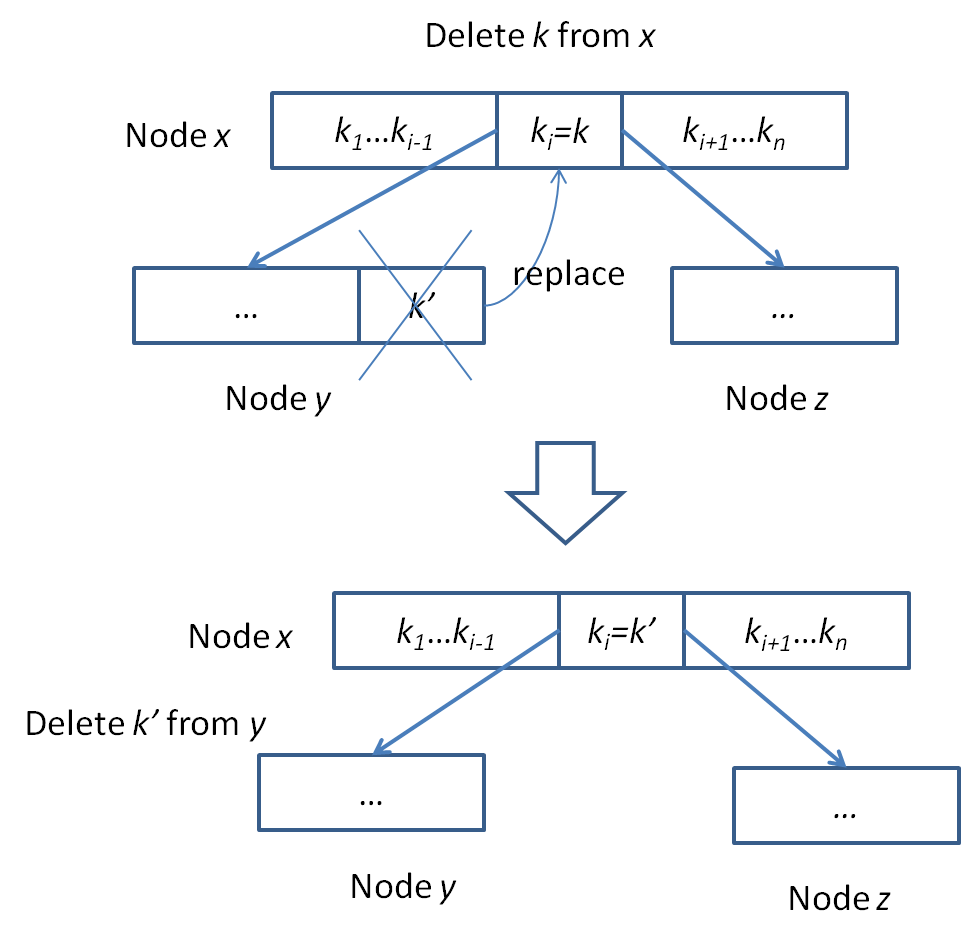
\includegraphics[scale=0.5]{img/btree-del-case2a.eps}
    \caption{case 2a. Replace and delete from predecessor.} \label{fig:btree-del-case2a}
  \end{center}
\end{figure}

\begin{figure}[htbp]
  \begin{center}
    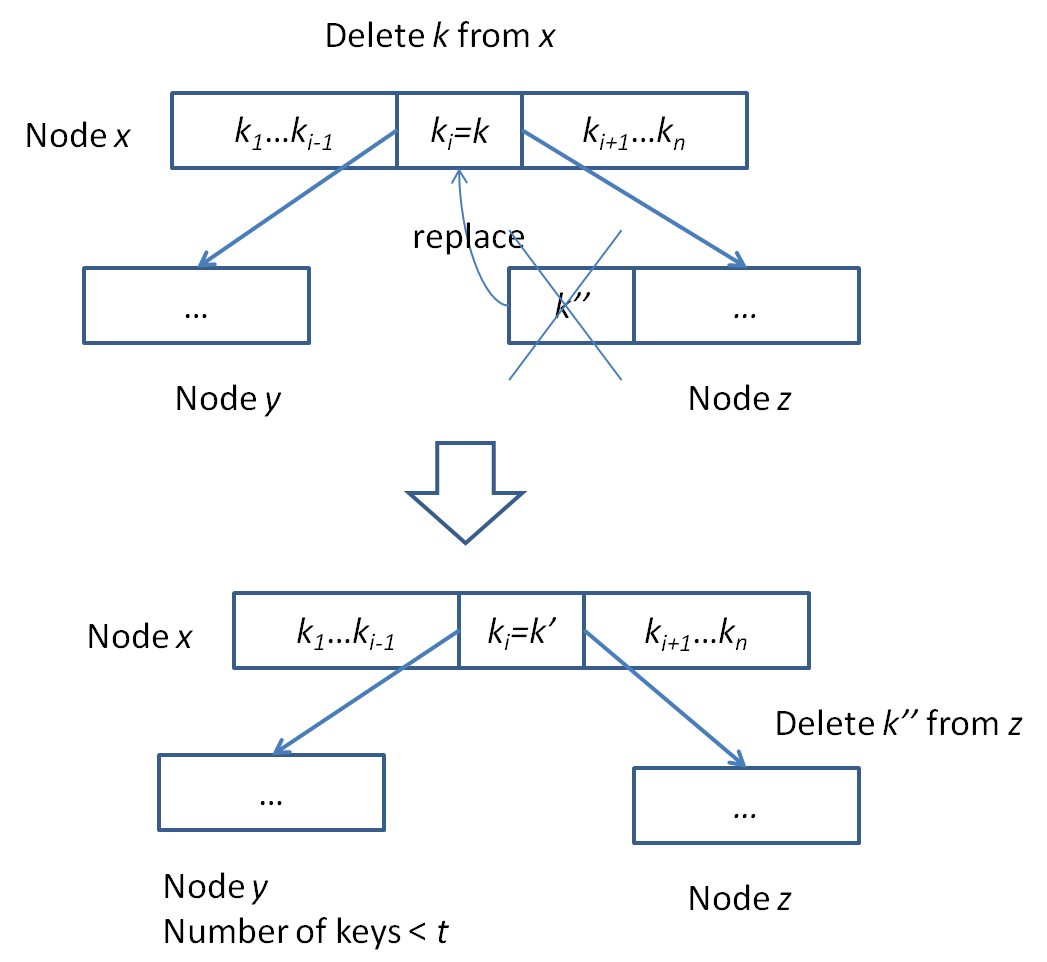
\includegraphics[scale=0.5]{img/btree-del-case2b.eps}
    \caption{case 2b. Replace and delete from successor.} \label{fig:btree-del-case2b}
  \end{center}
\end{figure}

\begin{figure}[htbp]
  \begin{center}
    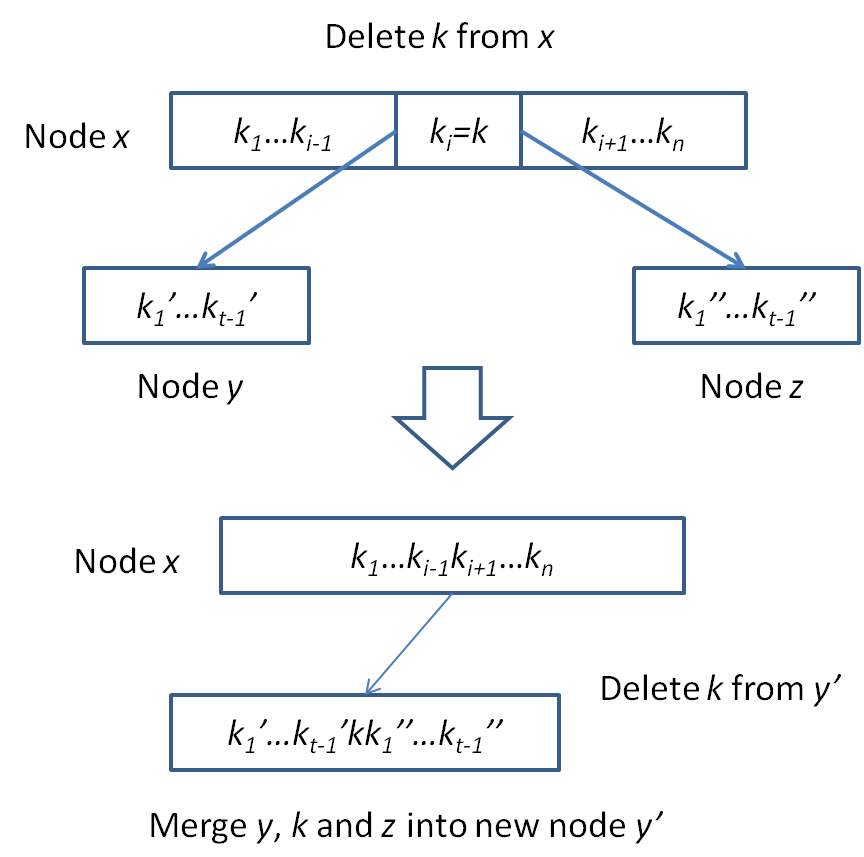
\includegraphics[scale=0.5]{img/btree-del-case2c.eps}
    \caption{case 2c. Merge and delete.} \label{fig:btree-del-case2c}
  \end{center}
\end{figure}

Note that although we use recursive way to delete keys in case 2, the 
resursion can be turned into pure imperative way. We'll show such
program in C++ implementation.

the last case states that, if $k$ can't be located in node $x$, the algorithm
need try to find a child node $c_i$ of $x$, so that sub-tree $c_i$ may 
contains $k$. Before the deletion is recursively applied in $c_i$, we
need be sure that there are at least $t$ keys in $c_i$. If there are
not enough keys, we need do the following adjustment.

\begin{itemize}
\item We check the two sibling of $c_i$, which are $c_{i-1}$ and $c_{i+1}$.
If either one of them contains enough keys (at least $t$ keys), we move
one key from $x$ down to $c_i$, and move one key from the sibling up to
$x$. Also we need move the relative child from the sibling to $c_i$.

This operation makes $c_i$ contains enough keys OK for deletion. we can
next try to delete $k$ from $c_i$ recursively.

\item In case neither one of the two siblings contains enough keys, we then 
merge $c_i$, a key from $x$, and either one of the sibling into a new
node, and do the deletion on this new node.
\end{itemize}

Case 3 is illustrated in figure \ref{fig:btree-del-case3a}, \ref{fig:btree-del-case3b}.

\begin{figure}[htbp]
  \begin{center}
    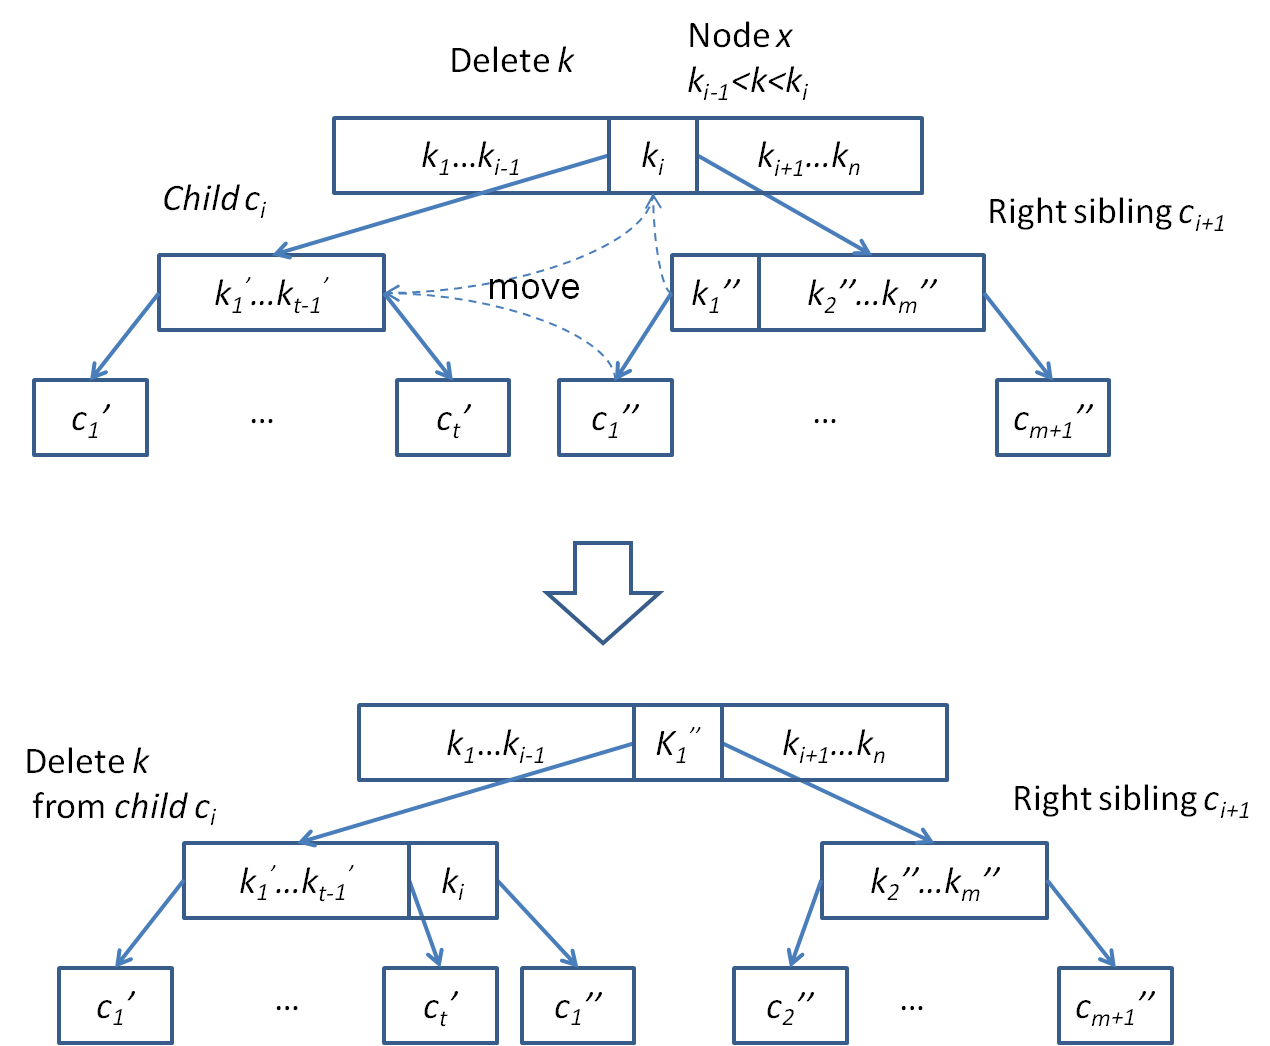
\includegraphics[scale=0.5]{img/btree-del-case3a.eps}
    \caption{case 3a. Borrow from left sibling.} \label{fig:btree-del-case3a}
  \end{center}
\end{figure}

\begin{figure}[htbp]
  \begin{center}
    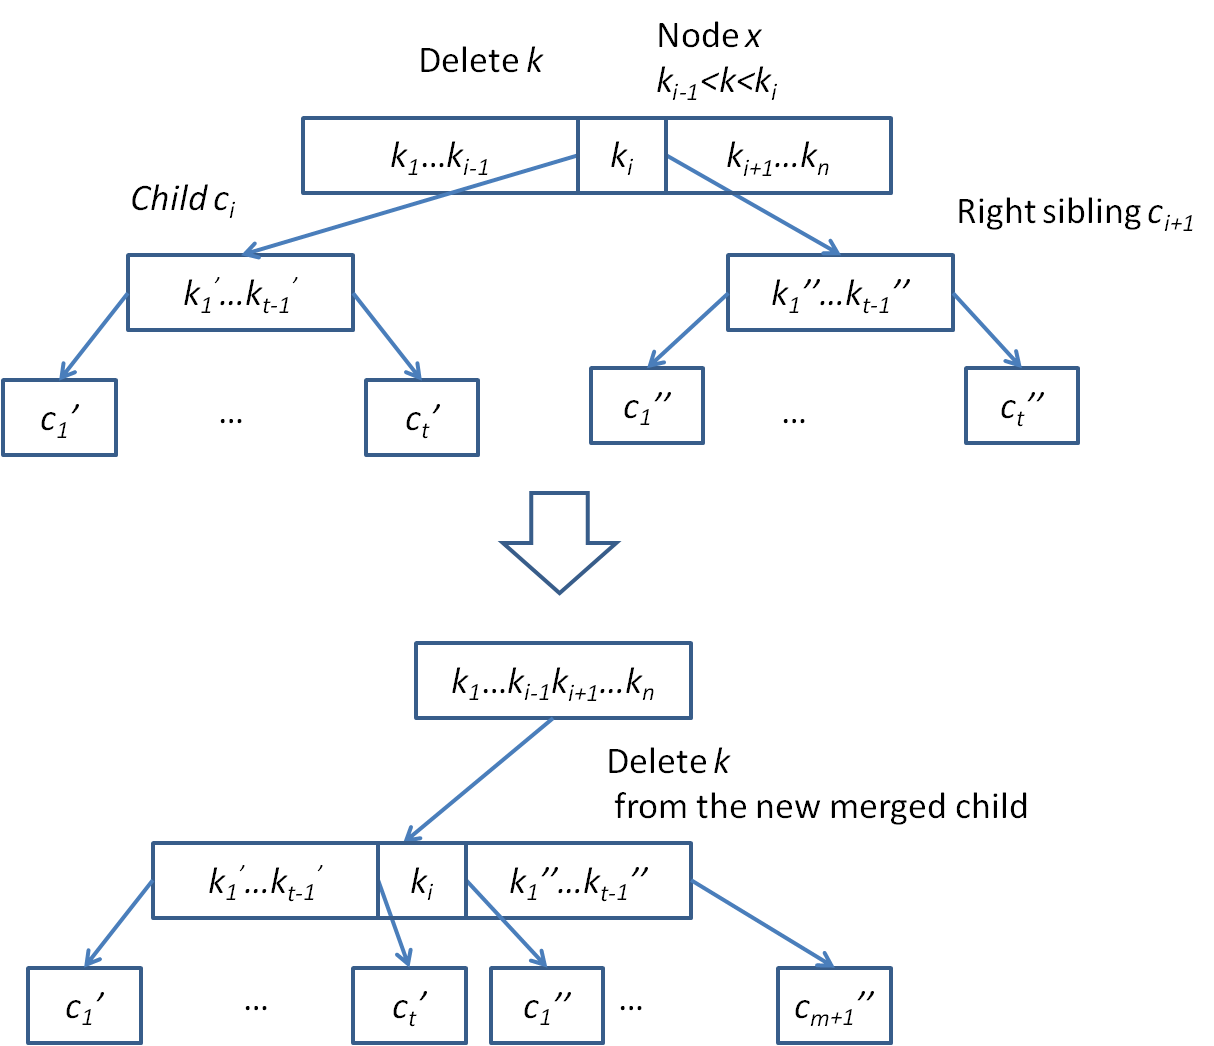
\includegraphics[scale=0.5]{img/btree-del-case3b.eps}
    \caption{case 3b. Borrow Merge and delete.} \label{fig:btree-del-case3b}
  \end{center}
\end{figure}

By implementing the above 3 cases into pseudo code, the B-tree delete algorithm
can be given as the following.

First there are some auxiliary functions to do some simple test and operations
on a B-tree.

\begin{algorithmic}[1]
\Function{CAN-DEL}{$T$}
  \State \Return number of keys of  $T \ge t$
\EndFunction
\end{algorithmic}

Function $CAN-DEL$ test if a B-tree node contains enough keys (no less than
$t$ keys).

\begin{algorithmic}[1]
\Procedure{MERGE-CHILDREN}{$T, i$} \Comment{Merge children $i$ and $i+1$}
  \State $x \leftarrow CHILDREN(T)[i]$
  \State $y \leftarrow CHILDREN(T)[i+1]$
  \State $APPEND(KEYS(x), KEYS(T)[i])$
  \State $CONCAT(KEYS(x), KEYS(y))$
  \State $CONCAT(CHILDREN(x), CHILDREN(y)$
  \State $REMOVE(KEYS(T), i)$
  \State $REMOVE(CHILDREN(T), i+1)$
\EndProcedure
\end{algorithmic}

Procedure $MERGE-CHILDREN$ merges the $i$-th child, the $i$-th key, 
and $i+1$-th child of node $T$ into a new child, and remove the 
$i$-th key and $i+1$-th child after merging.

With these helper functions, the main algorithm of B-tree deletion is described
as below.

\begin{algorithmic}[1]
\Function{B-TREE-DELETE}{$T, k$}
  \State $i \leftarrow 1$
  \While{$i <= LENGTH(KEYS(T))$}
    \If{$k = KEYS(T)[i]$}
      \If{$T$ is leaf} \Comment{case 1}
        \State $REMOVE(KYES(T), k)$
      \Else \Comment{case 2}
        \If{$CAN-DEL(CHILDREN(T)[i])$} \Comment{case 2a}
          \State $KEYS(T)[i] \leftarrow LAST-KEY(CHILDREN(T)[i])$
          \State $B-TREE-DELETE(CHILDREN(T)[i], KEYS(T)[i])$
        \ElsIf{$CAN-DEL(CHILDREN(T)[i+1])$} \Comment{case 2b}
          \State $KEYS(T)[i] \leftarrow FIRST-KEY(CHILDREN(T)[i+1])$
          \State $B-TREE-DELETE(CHILDREN(T)[i+1], KEYS(T)[i])$
        \Else \Comment{case 2c}
          \State $MERGE-CHILDREN(T, i)$
          \State $B-TREE-DELETE(CHILDREN(T)[i], k)$
          \If{$KEYS(T) = NIL$}
            \State $T \leftarrow CHILDREN(T)[i]$ \Comment{Shrinks height}
          \EndIf
        \EndIf
      \EndIf
      \State \Return $T$
    \ElsIf{$k < KEYS(T)[i]$}
      \State $BREAK$
    \Else
      \State $i \leftarrow i+1$
    \EndIf
  \EndWhile
  \Statex
  \If{$T$ is leaf}
    \State \Return $T$ \Comment{$k$ doesn't exist in $T$ at all}
  \EndIf
  \If{not $CAN-DEL(CHILDREN(T)[i])$}  \Comment{case 3}
    \If{$i>1$ and $CAN-DEL(CHILDREN(T)[i-1])$} \Comment{case 3a: left sibling}
      \State $INSERT(KEYS(CHILDREN(T)[i]), KEYS(T)[i-1])$
      \State $KEYS(T)[i-1] \leftarrow POP-BACK(KEYS(CHILDREN(T)[i-1]))$
      \If{$CHILDREN(T)[i]$ isn't leaf}
        \State $c \leftarrow POP-BACK(CHILDREN(CHILDREN(T)[i-1]))$
        \State $INSERT(CHILDREN(CHILDREN(T)[i]), c)$
      \EndIf
    \ElsIf{$i<=LENGTH(CHILDREN(T))$ and $CAN-DEL(CHILDREN(T)[i+1]$} \Comment{case 3a: right sibling}
      \State $APPEND(KEYS(CHILDREN(T)[i]), KEYS(T)[i])$
      \State $KEYS(T)[i] \leftarrow POP-FRONT(KEYS(CHILDREN(T)[i+1]))$
      \If{$CHILDREN(T)[i]$ isn't leaf}
        \State $c \leftarrow POP-FRONT(CHILDREN(CHILDREN(T)[i+1]))$
        \State $APPEND(CHILDREN(CHILDREN(T)[i]), c)$
      \EndIf
    \Else \Comment{case 3b}
      \If{$i>1$}
        \State $MERGE-CHILDREN(T, i-1)$
      \Else
        \State $MERGE-CHILDREN(T, i)$
      \EndIf
    \EndIf
  \EndIf
  \State $B-TREE-DELETE(CHILDREN(T)[i], k)$ \Comment {recursive delete}
  \If{$KEYS(T) = NIL$} \Comment {Shrinks height}
    \State $T \gets CHILDREN(T)[1]$
  \EndIf
  \State \Return $T$
\EndFunction
\end{algorithmic}

\subsubsection{Merge before deletion algorihm implemented in C++}
TODO:...

\subsubsection{Merge before deletion algorithm implemented in Python}
TODO:...

% ================================================================
%               Delete and fix method
% ================================================================

\subsection{Delete and fix method}

\subsubsection{Delete and fix algorithm implemented functionaly}

% ================================================================
%               Searching
% ================================================================
\section{Searching} 

\subsection{Imperative search algorithm}

\subsection{Functional search algorithm}

% ================================================================
%                 Short summary
% ================================================================
\section{Notes and short summary}


% ================================================================
%                 Appendix
% ================================================================
\section{Appendix} \label{appendix}
%\appendix
All programs provided along with this article are free for
downloading.

\subsection{Prerequisite software}
GNU Make is used for easy build some of the program. For C++ and ANSI C programs,
GNU GCC and G++ 3.4.4 are used. 
For Haskell programs GHC 6.10.4 is used
for building. For Python programs, Python 2.5 is used for testing, for
Scheme/Lisp program, MIT Scheme 14.9 is used.

all source files are put in one folder. Invoke 'make' or 'make all'
will build C++ and Haskell program. 

Run 'make Haskell' will separate build Haskell program. the executable
file is ``happ'' (with .exe
in Window like OS). It is also possible to run the program in GHCi.

\subsection{Tools}

Besides them, I use graphviz to draw most of the figures in this post. In order to
translate the Trie, Patrica and Suffix Tree output to dot language scripts. I wrote a python program.
it can be used like this.

\begin{verbatim}
st2dot -o filename.dot -t type "string"
\end{verbatim}

Where filename.dot is the output file for the dot script, type can be
either trie or tree, the default value is tree. it can generate suffix
Trie/tree from the string input and turns the tree/Trie into dot script.

This helper scripts can also be downloaded with this article.

download position: http://sites.google.com/site/algoxy/stree/stree.zip

\begin{thebibliography}{99}

\bibitem{CLRS}
Thomas H. Cormen, Charles E. Leiserson, Ronald L. Rivest and Clifford Stein. ``Introduction to Algorithms, Second Edition''. The MIT Press, 2001. ISBN: 0262032937.

\bibitem{wiki-b-tree}
B-tree, Wikipedia. http://en.wikipedia.org/wiki/B-tree

\bibitem{lxy-bst}
Liu Xinyu. ``Comparison of imperative and functional implementation of
binary search tree''. http://sites.google.com/site/algoxy/bstree

\bibitem{okasaki-rbtree}
Chris Okasaki. ``FUNCTIONAL PEARLS Red-Black Trees in a Functional Setting''. J. Functional Programming. 1998

\end{thebibliography}

\ifx\wholebook\relax \else
\end{document}
\fi
